\newpage
\begin{center}
  \textbf{\large АННОТАЦИЯ}
\end{center}

Один из методов косвенного обнаружения темной материи --- детектирование нейтринными обсерваториями потоков нейтрино, образующихся в результате аннигиляции темной материи, которая захватывается и накапливается  в гравитационном поле астрофизических объектов, таких как Солнце или Земля. На данный момент этот сигнал не обнаружен, что накладывает ограничения на сечение взаимодействия частиц темной материи с нуклоном. В данной работе, используя данные из IceCube, мы получим такие ограничения для случая неупругой темной материи, состоящей из основного и возбужденного состояния, для которой ограничения на сечения ослаблены по сравнению с упругой темной материей. 

Для вычисления ограничений необходимо найти число захваченных частиц темной материи, его распределение внутри небесного объекта на данный момент и темп аннигиляции. Для этого мы будем численно решать уравнение Больцмана, поскольку неупругая темная материя при некоторых разницах масс основного и возбужденного состояний не успевает прийти к термальному равновесию, что приводит к еще большему ослаблению ограничений на сечение.

\onehalfspacing
\setcounter{page}{2}

\newpage
\renewcommand{\contentsname}{\centerline{\large СОДЕРЖАНИЕ}}
\tableofcontents

\newpage
\begin{center}
  \textbf{\large ВВЕДЕНИЕ}
\end{center}
\addcontentsline{toc}{chapter}{ВВЕДЕНИЕ}


Одна из основных проблем современной космологии --- это проблема темной материи.  Темная материя --- это часть нерелятивисткой материи, находящейся во Вселенной, которая пока еще не регистрируется напрямую, однако участвует в гравитационном взаимодействии, в частности в расширении Вселенной и образовании структур. 


Наблюдения за астрономическими объектами и исследования анизотропии реликтового излучения позволяет найти основные параметры космологических моделей, такие как доля нерелятивистского вещества и барионной материи. Для современных космологических моделей доля вещества в настоящий момент составляет $\Omega_M = 0.2-0.3$, при этом доля барионной материи составляет всего $0.03-0.05$ \cite{Cao_2023}. Это означает, что большая часть вещества во Вселенной остается не объясненной на сегодняшний день наблюдаемой материей.

На наличие темной материи также указывают наблюдения скоростей звезд внутри галактик. Такие исследования позволяют найти распределение массы и плотность материи внутри галактики \cite{Radial_velocity_measurements}, \cite{Angular_Velocity}. Отношение измеренной таким образом гравитационной массы и массы наблюдаемого светимого вещества оказывается значительно больше единицы. Аналогичные исследования позволяют найти локальную плотность темной матери в Солнечной системе. Эта плотность равна $\rho_{DM} = 0.2 - 0.4 \, \text{ГэВ} \cdot \text{см}^{-3}$ \cite{palau2022oblateness}. В данной работе мы будем использовать значение  $\rho_{DM} = 0.4 \,\text{ГэВ} \cdot  	\text{см}^{-3}$.


Существуют различные способы объяснить явление темной материи. Так, в качестве темной материи могут быть массивные астрономические компактные объекты (первичные черные дыры с массой порядка $10-100M_{\odot}$). Такие объекты могут быть обнаружены с помощью измерения светимости и гравитационного линзирования, и на сегодняшний день наблюдения дают ограничения на их долю в массе нерелятивисткого вещества в районе $0.15-0.3$ \cite{Zumalac_rregui_2018}, \cite{Blaineau_2022}.
Также существуют различные модификации теории гравитации, которые могут объяснить кривые вращения или вклад материи в метрики без включения в модель новых частиц \cite{1984ApJ...286....7B}.


Наиболее распространенные модели темной материи предполагают наличие новых частиц вне Стандартной модели. В качестве кандидатов рассматривают, например, майорановские стерильные нейтрино \cite{Boyarsky_2019}, наличие которых может указать регистрация двойного безнейтринного $\beta$-распада или спектральных линий фотонов, возникающих при их распаде. 

Также, темной материей могут быть аксионы, призванные решить проблему сильного CP нарушения, которые могут осциллировать в фотоны в сильных электромагнитных полях \cite{adams2023axion}. Частицы темной материи появляются и в суперсимметричных расширениях Стандартной модели \cite{berezinsky1996dark}, так как из-за сохранения R-четности легчайшая частица-суперпартнер оказывается стабильной и может быть основой для массивных слабовзаимодействующих частиц, о которых будет идти речь далее.

Массивные слабовзаимодействующие частицы (WIMP) --- это частицы темной материи в широком диапазоне масс ($\text{МэВ}-\text{ТэВ}$). Предполагается, что эти частицы находились в термальном равновесии с остальной материей на ранних этапах эволюции Вселенной. Затем, при расширении Вселенной, когда темп аннигиляции становится меньше темпа расширения (постоянная Хаббла на соответствующий момент времени), эти частицы замораживаются, будучи нерелятивистскими. Соответствующая температура определяется соотношением \cite{Kolb:1990vq}: 
\begin{equation}
	x_f = \cfrac{m_{\chi} }{T_f} = \ln {\left(\cfrac{0.038 g_{\chi} M_{pl} m_{\chi}  \average{\sigma_{ann} v}}
		{\sqrt{g_* x_f}}\right)}
\end{equation}
где $g_{\chi}$ и $g_*$ --- степени свободы темной материи и релятивистского вещества, $M_{pl}$ --- масса Планка, $\average{\sigma_{ann} v} = \sigma_0$ --- среднее произведение сечения аннигиляции частиц темной материи и скорости. И доля темной материи, состоящей из этих частиц, равна: 
\begin{equation}
	\Omega{\chi} = \cfrac{\sn{1.9}{-27} x_f}{\sqrt{g_*} \sigma_0} \frac{cm^3}{s}
\end{equation}
При разумных параметрах ($x_f \approx 20, g_* \approx 80$), для объяснения сегодняшней плотности темной материи данным механизмом необходимо, чтобы $\sigma_0 \approx 10^{26} \text{см}^3\text{с}^{-1}$, что по порядку величины близко значениям, характерным для слабых взаимодействий.

Темная материя, находящаяся в галактическом гало, может быть обнаружена прямыми методами в низкофоновых экспериментах. Такой способ основан на детектировании отдачи при взаимодействии частиц темной материи с ядром \cite{Schumann_2019}. Наиболее известные эксперименты --- DAMA/LIBRA, COSINE-100, XENON100, XENON1T, CDMS, использующие в качестве мишени такие вещества, как NaI, Xe, Ge. На данный момент эти эксперименты не обнаружили значительного превышения сигнала над фоном, кроме DAMA/LIBRA, регистрирующий сигнал годовых модуляций, который свидетельствует о наличие темной материи \cite{Bernabei_2018}. Однако, эксперимент COSINE-100, имеющий ту же мишень (NaI), не подтвердил эти результаты \cite{Adhikari_2022}.

В данной работе рассматривается косвенный метод обнаружения темной материи, основанный на поиске продуктов аннигиляции частиц темной материи, захваченных небесными телами. Частицы темной материи взаимодействуют с частицами вещества, сосредоточенного в астрономических объектах, и передают им часть кинетической энергии. Это приводит к захвату темной материи в гравитационном потенциале небесного тела. В результате темная материя накапливается, что приводит к значительному усилению темпа аннигиляции. Таким образом создаются потоки нейтрино, которые возможно зарегистрировать в нейтринных обсерваториях  IceCube \cite{Aartsen_2017}, SuperKamiokande \cite{kamiokandecollaboration2015search}, ANTARES \cite{ADRIANMARTINEZ201669}. Для захвата частиц темной материи рассматриваются, как правило, Солнце \cite{1985ApJ...296..679P} или Земля \cite{1987ApJ...321..571G}. Для более легких частиц темной материи рассматривается Юпитер \cite{French_2022}, так как испарение на Юпитере значительно ниже. Отсутствие нейтринного сигнала дает ограничение на сечение взаимодействия с протоном $\sigma_{\chi p}$ (рис. \ref{graph:constr}) из предположения равновесия скорости захвата и скорости аннигиляции. 

\begin{figure}[!h]
	\begin{center}
		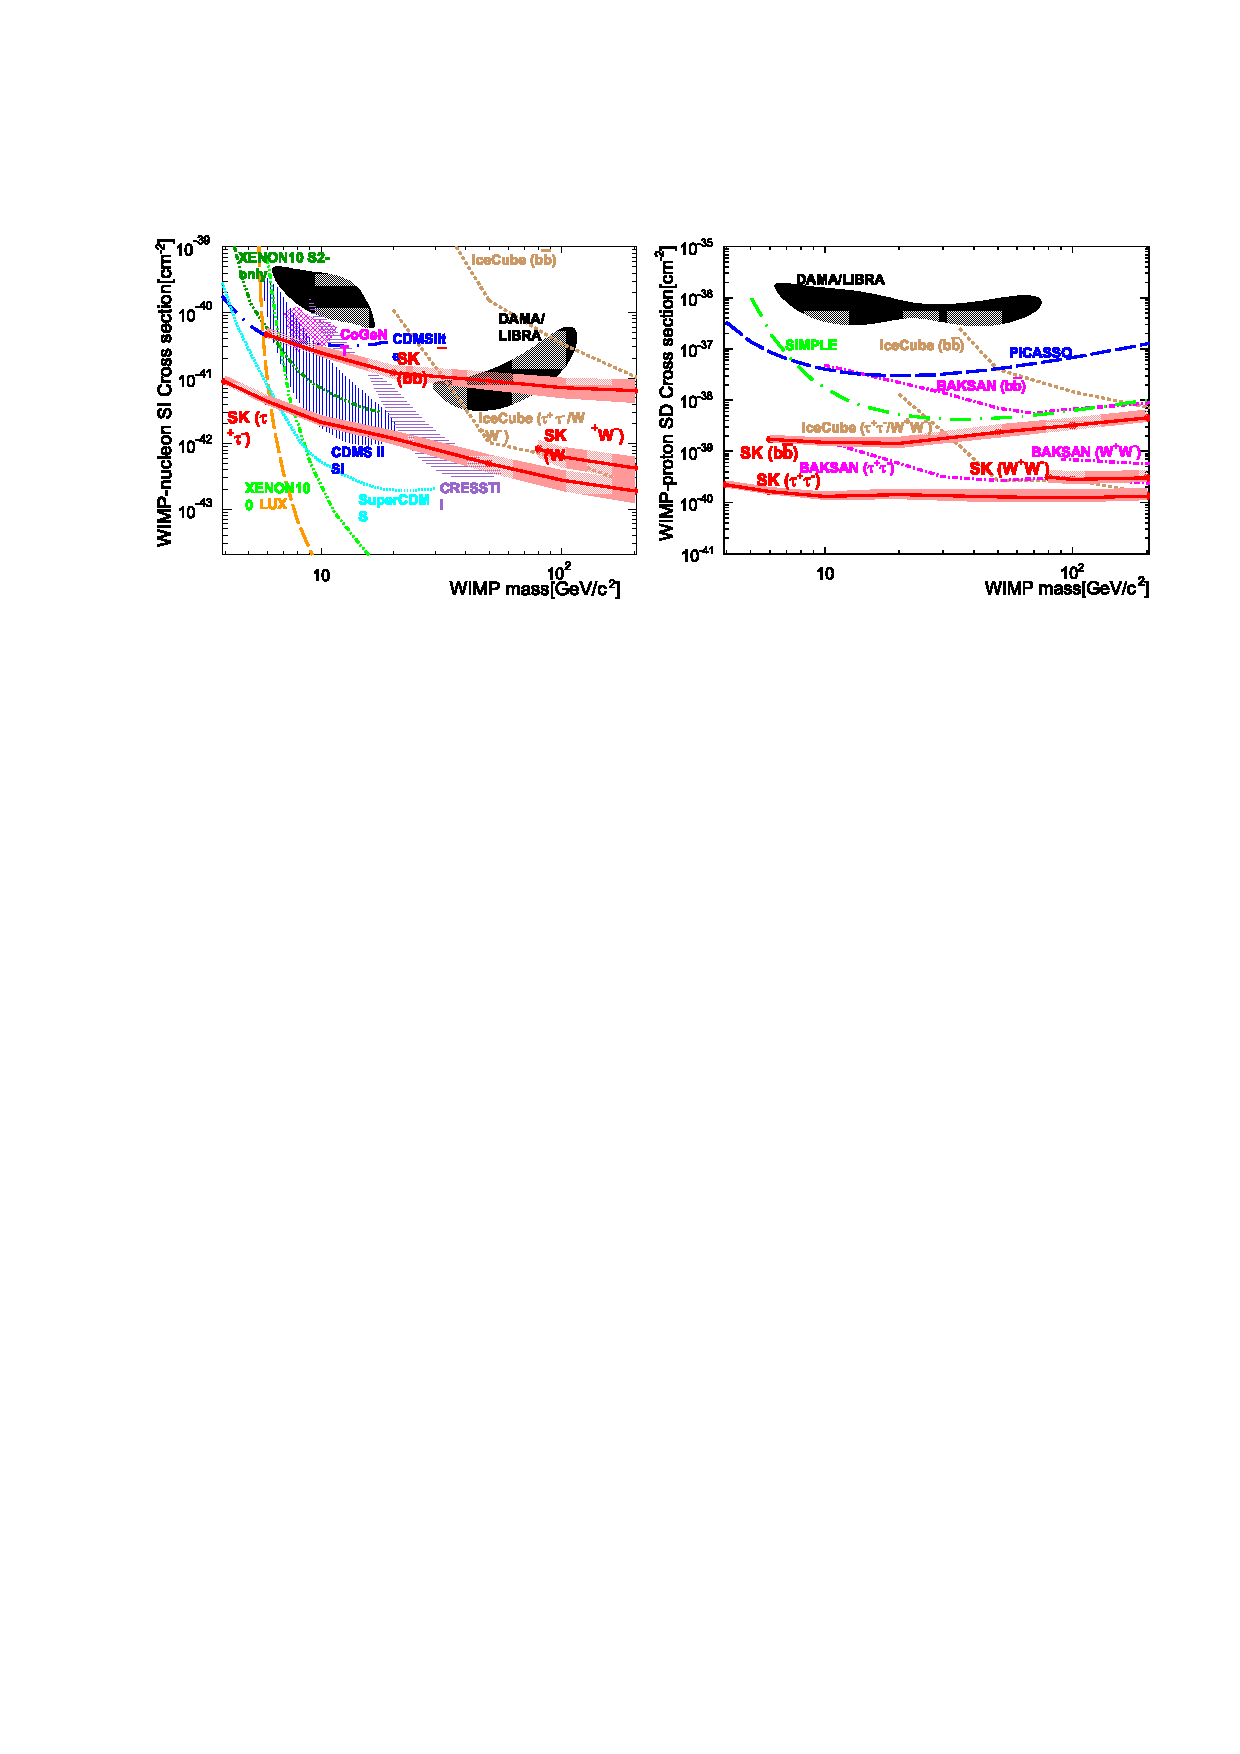
\includegraphics[scale=0.9]{images/SK_graphs.pdf}
	\end{center}
	\caption{Ограничения на сечение взаимодействия из разных экспериментов с протоном $\sigma_{\chi p}$. Слева --- для спин независимых взаимодействий, справа для спин зависимых взимодействий \cite{kamiokandecollaboration2015search}.}
	\label{graph:constr}
\end{figure}

Поскольку на данный момент ни прямыми, ни косвенными методами не удалось обнаружить частицы темной материи и многие простые модели исключены, создаются более сложные модели частиц темной материи.
В данной работе рассматривается двухкомпонентная неупругая темная материя, частица которой имеет основное $\chi$ и возбужденное состояние $\chi^*$ с массами $m_{\chi}$ и $m_{\chi}+\delta$, соответственно. Изначально такая модификация частиц темной материи была предложена для объяснения расхождений между экспериментом DAMA/LIBRA и CDMS \cite{PhysRevD.64.043502}, имеющих разную массу мишени, поскольку от нее зависит, будет ли при рассеянии преодолен энергетический порог $\delta$. Хотя результаты DAMA/LIBRA не смогли воспроизвестись на COSINE-100, такие модели могут ослабить ограничения на сечения, и поэтому представляют интерес.

Важным отличием неупругой темной материи является нетривиальная термализация. Если в упругом случае частицы приходят в больцмановское равновесие для интересных значений сечения, то неупругая темная материя может не успеть прийти в термальное равновесие с небесным телом \cite{Blennow_2018}. Поэтому термализация требует более детального анализа.

Целью данной работы является получение ограничения на сечения рассеяния частицы темной материи с учетом процессов термализации, исходя из данных IceCube.

